% Adapted from the documented scopes-library shorthand example in the local PGF manual.
\documentclass[border=2pt]{standalone}
\usepackage{tikz}
\usetikzlibrary{scopes}
\begin{document}
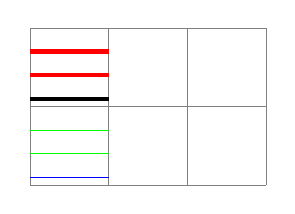
\begin{tikzpicture}
  \draw[help lines] (0,0) grid (3,2);
  { [ultra thick]
    { [red]
      \draw (0,1.7) -- (1,1.7);
      \draw (0,1.4) -- (1,1.4);
    }
    \draw (0,1.1) -- (1,1.1);
  }
  { [green]
    \draw (0,0.7) -- (1,0.7);
    \draw (0,0.4) -- (1,0.4);
    \draw[blue] (0,0.1) -- (1,0.1);
  }
\end{tikzpicture}
\end{document}
